% ═══════════════════════════════════════════════════════════════════════════════
% Chapter 4: Machine Learning Foundations for Biological AI
% Part II: The Intelligence Stack
% ═══════════════════════════════════════════════════════════════════════════════

\part{The Intelligence Stack}

\chapter{Machine Learning Foundations for Biological AI}
\label{ch:ml-foundations}

\chapterepigraph{A learning machine is a machine that can change its behavior in response to experience.}{After Alan Turing, 1950}

\noindent
Parts~I established that biology encodes, regulates, and evolves information through sophisticated computational mechanisms. This chapter begins Part~II by building the machine learning foundations needed to translate those biological principles into working AI systems. We cover neural networks, optimization, representation learning, and evolutionary algorithms---focusing specifically on the concepts that reappear in DOGMA's architecture.

This is not a comprehensive ML textbook (we recommend \citet{goodfellow2016} for that). Instead, it is a targeted introduction that equips the reader with the precise ML vocabulary and intuitions needed for the DOGMA chapters that follow.

% ───────────────────────────────────────────────────────────────────────────────
\section{The Learning Problem}
\label{sec:learning-problem}

\subsection{Supervised Learning as Function Approximation}

At its core, machine learning is about finding patterns in data. The simplest formulation is \emph{supervised learning}: given a dataset of input-output pairs, find a function that maps inputs to outputs.

\begin{dogmadef}[Supervised Learning]
Given a dataset $\mathcal{D} = \{(\mathbf{x}_i, y_i)\}_{i=1}^N$ of input-output pairs drawn from some unknown distribution $p(\mathbf{x}, y)$, find a function $f_\theta : \mathcal{X} \to \mathcal{Y}$ that minimizes expected loss:
\begin{equation}
\theta^* = \arg\min_\theta \; \mathbb{E}_{(\mathbf{x}, y) \sim p} \bigl[ \mathcal{L}(f_\theta(\mathbf{x}), y) \bigr],
\label{eq:erm}
\end{equation}
where $\mathcal{L}$ is a loss function and $\theta$ are learnable parameters. In practice, we approximate the expectation with the empirical mean over $\mathcal{D}$.
\end{dogmadef}

There are three crucial choices in any supervised learning setup: (1) the \emph{model class} (what family of functions $f_\theta$ can we represent?), (2) the \emph{loss function} (what does ``good'' mean?), and (3) the \emph{optimizer} (how do we search for $\theta^*$?). The rest of this chapter develops each of these in detail.

\paragraph{Worked example: DNA GC-content classification.} Suppose we want to classify DNA sequences of length 10 into ``GC-rich'' ($\geq 60\%$ G/C content) or ``GC-poor'' ($< 60\%$). Our input is a sequence like \texttt{ATCGGCTAGC}, represented as a vector $\mathbf{x} \in \{0,1\}^{40}$ using one-hot encoding (4 bases $\times$ 10 positions), and our output is a binary label $y \in \{0, 1\}$. We seek a function $f_\theta$ that predicts $y$ from $\mathbf{x}$. A simple approach is logistic regression: $f_\theta(\mathbf{x}) = \sigma(\mathbf{w}^\top \mathbf{x} + b)$, where $\sigma$ is the sigmoid function.

Let us trace through this concretely. For the sequence \texttt{ATCGGCTAGC}, the one-hot encoding assigns a 4-dimensional vector to each position: A$\to[1,0,0,0]$, T$\to[0,0,0,1]$, C$\to[0,1,0,0]$, G$\to[0,0,1,0]$. Concatenating all 10 positions yields a 40-dimensional binary vector. The GC content is $6/10 = 60\%$, so the label is $y = 1$ (GC-rich). If we initialize $\mathbf{w}$ so that the weights corresponding to G and C positions are positive ($+0.3$ each) and A and T positions are negative ($-0.2$ each), the pre-activation $z = \mathbf{w}^\top \mathbf{x} + b$ will be positive for GC-rich sequences, and $\sigma(z)$ will be close to 1. Training adjusts these weights to maximize classification accuracy on the training set.

\subsection{Loss Functions}

The choice of loss function $\mathcal{L}$ determines what ``good prediction'' means. The most common loss functions are:

\begin{center}
\renewcommand{\arraystretch}{1.2}
\begin{tabularx}{0.92\textwidth}{L{3.5cm} L{4.5cm} Y}
\toprule
\textbf{Loss Function} & \textbf{Formula} & \textbf{Use Case} \\
\midrule
Mean Squared Error (MSE) & $\frac{1}{N}\sum_{i=1}^N (y_i - \hat{y}_i)^2$ & Regression (continuous outputs) \\
Binary Cross-Entropy & $-\frac{1}{N}\sum_i [y_i \log \hat{y}_i + (1-y_i)\log(1-\hat{y}_i)]$ & Binary classification \\
Categorical Cross-Entropy & $-\frac{1}{N}\sum_i \sum_c y_{ic} \log \hat{y}_{ic}$ & Multi-class classification \\
Negative Log-Likelihood & $-\frac{1}{N}\sum_i \log p_\theta(y_i \mid \mathbf{x}_i)$ & General probabilistic models \\
\bottomrule
\end{tabularx}
\end{center}

\paragraph{Why cross-entropy and not MSE for classification?} For classification tasks, cross-entropy is preferred over MSE for two reasons. First, the gradient of cross-entropy with respect to the logits simplifies to $\hat{\mathbf{y}} - \mathbf{y}$ (as you will prove in Exercise~4.1), producing a gradient that is large when the prediction is wrong and small when it is right. MSE gradients, by contrast, can become very small near $\hat{y} = 0$ or $\hat{y} = 1$ due to the saturating sigmoid, slowing learning. Second, cross-entropy has an information-theoretic interpretation: it measures the extra bits needed to encode the true distribution using the predicted distribution, connecting machine learning to the information theory discussed in Chapter~\ref{ch:code-of-life}.

\paragraph{Worked example: cross-entropy for nucleotide prediction.} Suppose our model predicts the next nucleotide in a DNA sequence. The true next base is G, encoded as $\mathbf{y} = [0, 0, 1, 0]$ (for A, C, G, T). Our model predicts probabilities $\hat{\mathbf{y}} = [0.1, 0.2, 0.6, 0.1]$. The cross-entropy loss is:
\begin{equation}
\mathcal{L} = -(0 \cdot \log 0.1 + 0 \cdot \log 0.2 + 1 \cdot \log 0.6 + 0 \cdot \log 0.1) = -\log 0.6 \approx 0.511.
\end{equation}
A perfect prediction of $\hat{y}_G = 1.0$ would give $\mathcal{L} = 0$. A uniform prediction of $\hat{y}_G = 0.25$ would give $\mathcal{L} = -\log 0.25 \approx 1.386$. The loss measures how ``surprised'' the model is by the true answer.

\subsection{The Bias-Variance Tradeoff}

A fundamental tension in machine learning is between models that are too simple (high bias) and too complex (high variance).

\begin{dogmadef}[The Bias-Variance Decomposition]
The expected error of a model can be decomposed as:
\begin{equation}
\text{Error} = \underbrace{\text{Bias}^2}_{\substack{\text{systematic error from} \\ \text{model assumptions}}} + \underbrace{\text{Variance}}_{\substack{\text{sensitivity to} \\ \text{training data}}} + \underbrace{\text{Irreducible noise}}_{\substack{\text{inherent randomness} \\ \text{in the data}}}.
\end{equation}
\end{dogmadef}

\paragraph{Intuition.} Imagine fitting a curve to noisy data:
\begin{itemize}[leftmargin=1.5em]
  \item A straight line (linear model) may miss the true pattern (high bias, low variance).
  \item A degree-20 polynomial may fit every noise point (low bias, high variance).
  \item A degree-3 polynomial may capture the true pattern without overfitting (good tradeoff).
\end{itemize}

\paragraph{Why the tradeoff matters quantitatively.} Consider a concrete scenario. Suppose the true function is $f(x) = \sin(x)$ and we observe data with Gaussian noise $\epsilon \sim \mathcal{N}(0, 0.1^2)$. A linear model $\hat{f}(x) = ax + b$ has high bias (it cannot represent the curvature of sine) but low variance (the estimated line changes little between different training samples). A degree-15 polynomial has low bias (it can approximate $\sin(x)$ well) but high variance: with only 10 training points, the polynomial wiggles wildly between data points, and different training sets produce drastically different fits. A degree-3 polynomial $\hat{f}(x) = a_0 + a_1 x + a_2 x^2 + a_3 x^3$ provides a good tradeoff: the Taylor expansion of $\sin(x)$ is $x - x^3/6 + \cdots$, so degree 3 captures the dominant pattern while having few enough parameters to be stably estimated.

% TikZ diagram: Bias-Variance tradeoff
\begin{center}
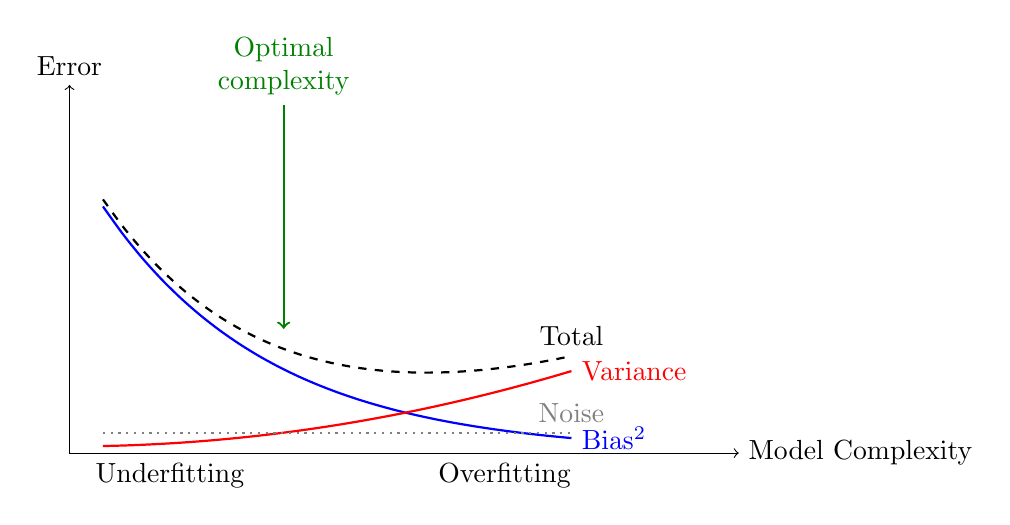
\begin{tikzpicture}[scale=0.85]
  % Axes
  \draw[->] (0,0) -- (10,0) node[right] {Model Complexity};
  \draw[->] (0,0) -- (0,5.5) node[above] {Error};

  % Bias^2 curve (decreasing)
  \draw[blue, thick, domain=0.5:7.5, smooth] plot (\x, {4.5*exp(-0.4*\x)})
    node[right, blue] {Bias$^2$};

  % Variance curve (increasing)
  \draw[red, thick, domain=0.5:7.5, smooth] plot (\x, {0.02*\x*\x + 0.1})
    node[right, red] {Variance};

  % Total error (sum)
  \draw[black, thick, dashed, domain=0.5:7.5, smooth] plot (\x, {4.5*exp(-0.4*\x) + 0.02*\x*\x + 0.1})
    node[above] {Total};

  % Irreducible noise
  \draw[gray, dotted, thick] (0.5, 0.3) -- (7.5, 0.3) node[above, gray] {Noise};

  % Optimal point
  \draw[<-, thick, green!50!black] (3.2, {4.5*exp(-0.4*3.2) + 0.02*3.2*3.2 + 0.1 + 0.3}) -- (3.2, 5.2)
    node[above, green!50!black, align=center] {Optimal\\complexity};

  % Labels
  \node[below, align=center] at (1.5, 0) {Underfitting};
  \node[below, align=center] at (6.5, 0) {Overfitting};
\end{tikzpicture}
\end{center}

\begin{bioinsight}[Biological Priors Reduce Variance]
DOGMA's structured architecture embeds biological priors---typed bases, region structure, regulatory logic---that constrain the hypothesis space. This is analogous to choosing a degree-3 polynomial when you know the underlying process is smooth: the prior reduces variance without excessive bias, because the structure matches the true data-generating process. In contrast, a flat transformer must discover all structure from data alone, requiring more data to achieve the same generalization.
\end{bioinsight}

\subsection{Unsupervised and Self-Supervised Learning}

Not all learning requires labeled data. In \emph{unsupervised learning}, the model discovers structure in unlabeled data (clustering, dimensionality reduction). In \emph{self-supervised learning}, the model creates its own supervisory signal from the data structure.

The dominant self-supervised paradigm for language models is \emph{next-token prediction}:
\begin{equation}
\mathcal{L}_{\text{LM}}(\theta) = -\sum_{t=1}^{T} \log p_\theta(x_t \mid x_1, \ldots, x_{t-1}).
\label{eq:lm-loss}
\end{equation}

This objective requires no human-labeled data---the text itself provides the supervision. The same principle applies to genomic sequences: predicting the next nucleotide given preceding context is a natural self-supervised objective for DNA language models (Chapter~\ref{ch:bio-foundation-models}).

\paragraph{Why self-supervised learning is so powerful.} The key advantage is \emph{data efficiency at the labeling stage}. Consider genomic data: we have billions of base pairs of sequenced DNA, but only a tiny fraction has been functionally annotated. Self-supervised pre-training on raw sequence data learns representations that capture sequence grammar, motif structure, and evolutionary constraints---all without a single label. These pre-trained representations can then be fine-tuned with a small number of labeled examples for specific tasks like promoter prediction or variant effect classification. This \emph{pre-train then fine-tune} paradigm is the foundation of modern biological AI.

\paragraph{Other self-supervised objectives.}
\begin{itemize}[leftmargin=1.5em]
  \item \textbf{Masked language modeling (MLM):} Randomly mask tokens and predict them from surrounding context. Used in BERT \citep{devlin2019} and DNABERT \citep{ji2021dnabert}. For example, given ``ATG\texttt{[MASK]}GC'', the model must predict that the masked token is most likely C or T based on context.
  \item \textbf{Contrastive learning:} Learn embeddings where similar items are close and dissimilar items are far. Used in protein representation learning \citep{lin2023}. The objective pulls together embeddings of augmented views of the same protein while pushing apart embeddings of different proteins.
  \item \textbf{Denoising:} Corrupt input and train the model to reconstruct the original. Used in denoising autoencoders and diffusion models. For DNA, corruption might involve random base substitutions, and the model learns to ``correct'' them.
\end{itemize}

% ───────────────────────────────────────────────────────────────────────────────
\section{Neural Networks from First Principles}
\label{sec:neural-networks}

\subsection{The Perceptron: A Single Neuron}

The simplest neural network is a single neuron (perceptron), which computes a weighted sum of its inputs, adds a bias, and applies a nonlinear activation function:

\begin{equation}
y = \phi(\mathbf{w}^\top \mathbf{x} + b) = \phi\!\left(\sum_{i=1}^d w_i x_i + b\right).
\end{equation}

The weights $\mathbf{w}$ determine how much each input contributes to the output, and the bias $b$ shifts the decision boundary. Together, $\mathbf{w}$ and $b$ define a hyperplane in $d$-dimensional space: the neuron outputs different values on each side of this hyperplane.

% TikZ diagram: Single neuron
\begin{center}
\begin{tikzpicture}[
    node distance=1.5cm,
    neuron/.style={circle, draw, minimum size=1cm, thick},
    input/.style={circle, draw, minimum size=0.6cm, fill=blue!10},
    >=stealth
]
  % Input nodes
  \node[input] (x1) at (0, 2.5) {$x_1$};
  \node[input] (x2) at (0, 1.0) {$x_2$};
  \node[input] (x3) at (0, -0.5) {$x_3$};
  \node at (0, -1.5) {$\vdots$};
  \node[input] (xd) at (0, -2.5) {$x_d$};

  % Bias node
  \node[input, fill=orange!15] (b) at (0, 4.0) {$1$};

  % Neuron
  \node[neuron, fill=green!10] (n) at (3.5, 0.5) {$\sum$};

  % Activation
  \node[neuron, fill=yellow!15] (phi) at (6.0, 0.5) {$\phi$};

  % Output
  \node[right=1cm of phi] (y) {$y$};

  % Weights
  \draw[->, thick] (x1) -- node[above, sloped, font=\small] {$w_1$} (n);
  \draw[->, thick] (x2) -- node[above, sloped, font=\small] {$w_2$} (n);
  \draw[->, thick] (x3) -- node[above, sloped, font=\small] {$w_3$} (n);
  \draw[->, thick] (xd) -- node[below, sloped, font=\small] {$w_d$} (n);
  \draw[->, thick, orange!70!black] (b) -- node[above, sloped, font=\small] {$b$} (n);

  % Sum to activation
  \draw[->, thick] (n) -- node[above, font=\small] {$z$} (phi);

  % Output
  \draw[->, thick] (phi) -- (y);

  % Label
  \node[below=0.3cm of n, font=\footnotesize, align=center] {Weighted\\sum};
  \node[below=0.3cm of phi, font=\footnotesize, align=center] {Non-\\linearity};
\end{tikzpicture}
\end{center}

\paragraph{Worked example.} Consider a neuron with 3 inputs ($d=3$), weights $\mathbf{w} = [0.5, -0.3, 0.8]$, bias $b = 0.1$, and ReLU activation $\phi(z) = \max(0, z)$. For input $\mathbf{x} = [1.0, 2.0, 0.5]$:
\begin{align}
z &= 0.5 \times 1.0 + (-0.3) \times 2.0 + 0.8 \times 0.5 + 0.1 \\
  &= 0.5 - 0.6 + 0.4 + 0.1 = 0.4, \\
y &= \max(0, 0.4) = 0.4.
\end{align}

If instead the input were $\mathbf{x} = [0.1, 2.0, 0.5]$, we would get $z = 0.05 - 0.6 + 0.4 + 0.1 = -0.05$, and $y = \max(0, -0.05) = 0$. The neuron is ``off'' for this input---ReLU has completely silenced it. This sparsity (many neurons outputting exactly zero) is a key property of ReLU networks and contributes to computational efficiency.

A single perceptron can only represent \emph{linear decision boundaries}. It can compute AND and OR but \emph{cannot} compute XOR---this limitation motivated the development of multi-layer networks.

\begin{center}
\renewcommand{\arraystretch}{1.1}
\begin{tabular}{cccccc}
\toprule
$x_1$ & $x_2$ & AND & OR & XOR & NAND \\
\midrule
0 & 0 & 0 & 0 & 0 & 1 \\
0 & 1 & 0 & 1 & 1 & 1 \\
1 & 0 & 0 & 1 & 1 & 1 \\
1 & 1 & 1 & 1 & 0 & 0 \\
\bottomrule
\end{tabular}
\end{center}

AND and OR are linearly separable (a single line separates the 0s from the 1s), but XOR is not. This is the historical motivation for \emph{deep} networks.

\subsection{Activation Functions}

The activation function $\phi$ introduces nonlinearity, enabling the network to learn complex patterns. Without nonlinearity, a stack of linear layers would collapse into a single linear transformation. To see why, note that if $f_1(\mathbf{x}) = \mathbf{W}_1 \mathbf{x} + \mathbf{b}_1$ and $f_2(\mathbf{x}) = \mathbf{W}_2 \mathbf{x} + \mathbf{b}_2$, then $f_2(f_1(\mathbf{x})) = \mathbf{W}_2(\mathbf{W}_1 \mathbf{x} + \mathbf{b}_1) + \mathbf{b}_2 = (\mathbf{W}_2 \mathbf{W}_1)\mathbf{x} + (\mathbf{W}_2 \mathbf{b}_1 + \mathbf{b}_2)$, which is just another linear function. No matter how many linear layers you stack, the result is equivalent to a single linear layer.

\begin{center}
\renewcommand{\arraystretch}{1.3}
\begin{tabularx}{0.95\textwidth}{L{2.5cm} L{4cm} L{3.5cm} Y}
\toprule
\textbf{Function} & \textbf{Formula} & \textbf{Range} & \textbf{Properties} \\
\midrule
Sigmoid & $\sigma(z) = \frac{1}{1+e^{-z}}$ & $(0, 1)$ & Smooth, saturates at extremes; vanishing gradient problem \\
Tanh & $\tanh(z) = \frac{e^z - e^{-z}}{e^z + e^{-z}}$ & $(-1, 1)$ & Zero-centered; still saturates \\
ReLU & $\max(0, z)$ & $[0, \infty)$ & Fast, sparse; ``dead neuron'' problem \\
Leaky ReLU & $\max(\alpha z, z)$, $\alpha \ll 1$ & $(-\infty, \infty)$ & Fixes dead neurons \\
GELU & $z \cdot \Phi(z)$ & $\approx (-0.17, \infty)$ & Smooth ReLU; used in transformers \\
Swish & $z \cdot \sigma(z)$ & $\approx (-0.28, \infty)$ & Self-gated; strong empirical performance \\
\bottomrule
\end{tabularx}
\end{center}

\paragraph{The vanishing gradient problem in detail.} Sigmoid and tanh saturate for large $|z|$: when $z = 10$, $\sigma'(10) \approx 0.0000454$. During backpropagation, gradients are multiplied through layers, so if each layer contributes a factor near zero, the gradient shrinks exponentially. For a network with $L$ layers, the gradient at the first layer is proportional to $\prod_{\ell=1}^{L} \sigma'(z^{(\ell)})$. If each factor is $0.25$ (the maximum of $\sigma'$), then after just 10 layers: $0.25^{10} \approx 9.5 \times 10^{-7}$. This makes training deep networks with sigmoid activations extremely difficult.

ReLU solves this by having a derivative of exactly 1 for $z > 0$, allowing gradients to flow unchanged through active neurons. The cost is the ``dead neuron'' problem: if a neuron's pre-activation $z$ is always negative for all training inputs, the gradient is always zero and the neuron can never recover. Leaky ReLU mitigates this by using a small positive slope $\alpha$ (typically 0.01) for negative inputs.

\begin{bioinsight}[Activation Functions and Biological Neurons]
Biological neurons fire when their membrane potential exceeds a threshold---a process well approximated by the sigmoid function. However, real neurons exhibit much richer dynamics: refractory periods, spike-rate adaptation, bursting patterns. DOGMA's regulatory activation weights $\rho_i$ generalize simple thresholding to context-dependent, multi-factor activation, more closely mirroring biological reality.
\end{bioinsight}

\subsection{Multi-Layer Perceptrons (MLPs)}

A \emph{multi-layer perceptron} (MLP) composes multiple layers of neurons:
\begin{equation}
\mathbf{h}^{(\ell)} = \phi^{(\ell)}\bigl(\mathbf{W}^{(\ell)} \mathbf{h}^{(\ell-1)} + \mathbf{b}^{(\ell)}\bigr), \quad \ell = 1, \ldots, L.
\end{equation}

Here, $\mathbf{h}^{(0)} = \mathbf{x}$ is the input, $\mathbf{W}^{(\ell)} \in \mathbb{R}^{d_\ell \times d_{\ell-1}}$ is the weight matrix connecting layer $\ell-1$ to layer $\ell$, $\mathbf{b}^{(\ell)} \in \mathbb{R}^{d_\ell}$ is the bias vector, and $d_\ell$ is the width (number of neurons) of layer $\ell$. The total number of learnable parameters is $\sum_{\ell=1}^{L} (d_\ell \times d_{\ell-1} + d_\ell)$.

\paragraph{Worked example: 2-layer MLP for XOR.} We solve XOR using a network with 2 inputs, a hidden layer of 2 neurons (ReLU activation), and 1 output neuron (sigmoid activation):
\begin{align}
\text{Hidden layer:} \quad \mathbf{W}^{(1)} &= \begin{bmatrix} 1 & 1 \\ 1 & 1 \end{bmatrix}, \quad \mathbf{b}^{(1)} = \begin{bmatrix} 0 \\ -1 \end{bmatrix} \\
\text{Output layer:} \quad \mathbf{w}^{(2)} &= \begin{bmatrix} 1 \\ -2 \end{bmatrix}, \quad b^{(2)} = 0
\end{align}

Let us verify all four cases:
\begin{center}
\renewcommand{\arraystretch}{1.2}
\begin{tabular}{cc|cc|c|c}
\toprule
$x_1$ & $x_2$ & $h_1 = \text{ReLU}(x_1 + x_2)$ & $h_2 = \text{ReLU}(x_1 + x_2 - 1)$ & $z = h_1 - 2h_2$ & $\hat{y} = \sigma(z)$ \\
\midrule
0 & 0 & 0 & 0 & 0 & 0.50 \\
0 & 1 & 1 & 0 & 1 & 0.73 \\
1 & 0 & 1 & 0 & 1 & 0.73 \\
1 & 1 & 2 & 1 & 0 & 0.50 \\
\bottomrule
\end{tabular}
\end{center}

The network outputs high values ($0.73$) for XOR=1 cases and $0.5$ for XOR=0 cases. With further weight tuning (e.g., scaling $\mathbf{w}^{(2)}$ by a factor of 10), the separation becomes sharper. The key insight: the hidden layer creates a \emph{new representation} in which the XOR problem becomes linearly separable. Neuron $h_1$ detects ``at least one input is 1'' and neuron $h_2$ detects ``both inputs are 1''; the output layer then computes ``$h_1$ but not $h_2$.''

\begin{theorem}[Universal Approximation \citep{goodfellow2016}]
A feedforward network with a single hidden layer of sufficient width can approximate any continuous function on a compact domain to arbitrary accuracy.
\end{theorem}

The theorem guarantees \emph{existence} but says nothing about \emph{efficiency}. Deep networks achieve the same approximation quality with exponentially fewer parameters than shallow ones for many function classes---this is why depth matters.

\paragraph{Why depth helps: a counting argument.} A function that requires $2^n$ neurons in a single hidden layer may require only $O(n)$ neurons distributed across $O(n)$ layers. For example, computing the parity of $n$ binary inputs requires exponentially many neurons in one layer but only $n-1$ neurons across $\log_2 n$ layers of XOR gates.

% ───────────────────────────────────────────────────────────────────────────────
\section{Training Neural Networks}
\label{sec:training}

\subsection{Backpropagation: Computing Gradients Efficiently}

Parameters are optimized via gradient descent, and the gradient of the loss with respect to each parameter is computed efficiently by \emph{backpropagation}---application of the chain rule through the computational graph.

\paragraph{The chain rule in action.} Consider a simple 2-layer network: $z_1 = w_1 x$, $h = \phi(z_1)$, $z_2 = w_2 h$, $\hat{y} = \sigma(z_2)$, $\mathcal{L} = -[y \log \hat{y} + (1-y)\log(1-\hat{y})]$. The gradient with respect to $w_1$ is:
\begin{equation}
\frac{\partial \mathcal{L}}{\partial w_1} = \frac{\partial \mathcal{L}}{\partial \hat{y}} \cdot \frac{\partial \hat{y}}{\partial z_2} \cdot \frac{\partial z_2}{\partial h} \cdot \frac{\partial h}{\partial z_1} \cdot \frac{\partial z_1}{\partial w_1}.
\end{equation}

Each factor in this chain is a simple local derivative. Backpropagation computes all gradients in a single backward pass through the network, with computational cost proportional to the forward pass.

% TikZ diagram: Computation graph for backpropagation
\begin{center}
\begin{tikzpicture}[
    node distance=2cm,
    box/.style={rectangle, draw, rounded corners, minimum width=1.4cm, minimum height=0.8cm, thick, fill=blue!5},
    param/.style={rectangle, draw, rounded corners, minimum width=1.2cm, minimum height=0.7cm, thick, fill=orange!10},
    >=stealth
]
  % Forward pass nodes
  \node[param] (x) {$x$};
  \node[param, below=0.7cm of x] (w1) {$w_1$};
  \node[box, right=1.5cm of x] (z1) {$z_1 = w_1 x$};
  \node[box, right=1.5cm of z1] (h) {$h = \phi(z_1)$};
  \node[param, below=0.7cm of h] (w2) {$w_2$};
  \node[box, right=1.5cm of h] (z2) {$z_2 = w_2 h$};
  \node[box, right=1.5cm of z2] (yhat) {$\hat{y} = \sigma(z_2)$};
  \node[box, right=1.5cm of yhat] (L) {$\mathcal{L}$};

  % Forward arrows
  \draw[->, thick, blue!60] (x) -- (z1);
  \draw[->, thick, blue!60] (w1) -- (z1);
  \draw[->, thick, blue!60] (z1) -- (h);
  \draw[->, thick, blue!60] (h) -- (z2);
  \draw[->, thick, blue!60] (w2) -- (z2);
  \draw[->, thick, blue!60] (z2) -- (yhat);
  \draw[->, thick, blue!60] (yhat) -- (L);

  % Backward arrows (below, dashed red)
  \draw[<-, thick, red!70, dashed] ([yshift=-0.4cm]z1.east) -- node[below, font=\scriptsize, red!70] {$\frac{\partial h}{\partial z_1}$} ([yshift=-0.4cm]h.west);
  \draw[<-, thick, red!70, dashed] ([yshift=-0.4cm]h.east) -- node[below, font=\scriptsize, red!70] {$\frac{\partial z_2}{\partial h}$} ([yshift=-0.4cm]z2.west);
  \draw[<-, thick, red!70, dashed] ([yshift=-0.4cm]z2.east) -- node[below, font=\scriptsize, red!70] {$\frac{\partial \hat{y}}{\partial z_2}$} ([yshift=-0.4cm]yhat.west);
  \draw[<-, thick, red!70, dashed] ([yshift=-0.4cm]yhat.east) -- node[below, font=\scriptsize, red!70] {$\frac{\partial \mathcal{L}}{\partial \hat{y}}$} ([yshift=-0.4cm]L.west);

  % Labels
  \node[above=0.2cm of z1, blue!60, font=\footnotesize] {Forward};
  \node[below=0.6cm of z2, red!70, font=\footnotesize] {Backward};
\end{tikzpicture}
\end{center}

\paragraph{Step-by-step backpropagation example.} Let $x = 2$, $w_1 = 0.5$, $w_2 = 1.0$, $y = 1$ (true label), and $\phi = \text{ReLU}$:
\begin{enumerate}[leftmargin=1.5em]
  \item \textbf{Forward pass:} $z_1 = 0.5 \times 2 = 1.0$; $h = \max(0, 1.0) = 1.0$; $z_2 = 1.0 \times 1.0 = 1.0$; $\hat{y} = \sigma(1.0) = 0.731$.
  \item \textbf{Loss:} $\mathcal{L} = -\log(0.731) = 0.313$.
  \item \textbf{Backward pass:}
  \begin{itemize}
    \item $\frac{\partial \mathcal{L}}{\partial \hat{y}} = -\frac{y}{\hat{y}} = -\frac{1}{0.731} = -1.368$
    \item $\frac{\partial \hat{y}}{\partial z_2} = \hat{y}(1-\hat{y}) = 0.731 \times 0.269 = 0.197$
    \item $\frac{\partial \mathcal{L}}{\partial z_2} = -1.368 \times 0.197 = -0.269$ (this is $\hat{y} - y = 0.731 - 1$)
    \item $\frac{\partial z_2}{\partial w_2} = h = 1.0$, so $\frac{\partial \mathcal{L}}{\partial w_2} = -0.269 \times 1.0 = -0.269$
    \item $\frac{\partial z_2}{\partial h} = w_2 = 1.0$, $\frac{\partial h}{\partial z_1} = 1$ (ReLU derivative for $z_1 > 0$)
    \item $\frac{\partial \mathcal{L}}{\partial w_1} = -0.269 \times 1.0 \times 1 \times x = -0.269 \times 2 = -0.538$
  \end{itemize}
  \item \textbf{Update:} With learning rate $\eta = 0.1$: $w_1 \leftarrow 0.5 - 0.1 \times (-0.538) = 0.554$; $w_2 \leftarrow 1.0 - 0.1 \times (-0.269) = 1.027$.
\end{enumerate}

Both weights increased, which will push $\hat{y}$ closer to $y = 1$ on the next forward pass. Let us verify: with the updated weights, the forward pass gives $z_1 = 0.554 \times 2 = 1.108$, $h = 1.108$, $z_2 = 1.027 \times 1.108 = 1.138$, $\hat{y} = \sigma(1.138) = 0.757$. Indeed, $\hat{y}$ has moved from $0.731$ to $0.757$, closer to the target $y=1$, and the loss decreased from $0.313$ to $-\log(0.757) = 0.278$.

\subsection{Gradient Descent Variants}

The basic gradient descent update rule is:
\begin{equation}
\theta \leftarrow \theta - \eta \nabla_\theta \mathcal{L}(\theta),
\end{equation}
where $\eta$ is the learning rate. In practice, several variants improve convergence:

\begin{center}
\renewcommand{\arraystretch}{1.2}
\begin{tabularx}{0.95\textwidth}{L{3cm} Y L{3cm}}
\toprule
\textbf{Optimizer} & \textbf{Key Idea} & \textbf{Update Rule (simplified)} \\
\midrule
SGD & Random mini-batch gradient estimates & $\theta \leftarrow \theta - \eta \hat{\nabla}\mathcal{L}$ \\
SGD + Momentum & Accumulate past gradients to smooth updates & $\mathbf{v} \leftarrow \beta \mathbf{v} + \hat{\nabla}\mathcal{L}$; $\theta \leftarrow \theta - \eta \mathbf{v}$ \\
AdaGrad & Per-parameter adaptive learning rates & $\theta_i \leftarrow \theta_i - \frac{\eta}{\sqrt{G_i + \epsilon}} \hat{\nabla}_i$ \\
Adam & Adaptive moments: combines momentum + AdaGrad & $\theta \leftarrow \theta - \eta \frac{\hat{m}}{\sqrt{\hat{v}} + \epsilon}$ \\
\bottomrule
\end{tabularx}
\end{center}

\paragraph{Worked example: gradient descent on a simple function.} To build intuition, consider minimizing $f(\theta) = (\theta - 3)^2$ starting from $\theta_0 = 0$ with learning rate $\eta = 0.2$. The gradient is $f'(\theta) = 2(\theta - 3)$.

\begin{center}
\renewcommand{\arraystretch}{1.15}
\begin{tabular}{c|c|c|c|c}
\toprule
\textbf{Step} $t$ & $\theta_t$ & $f(\theta_t)$ & $f'(\theta_t)$ & $\theta_{t+1} = \theta_t - 0.2 \cdot f'(\theta_t)$ \\
\midrule
0 & 0.000 & 9.000 & $-6.000$ & 1.200 \\
1 & 1.200 & 3.240 & $-3.600$ & 1.920 \\
2 & 1.920 & 1.166 & $-2.160$ & 2.352 \\
3 & 2.352 & 0.420 & $-1.296$ & 2.611 \\
4 & 2.611 & 0.151 & $-0.778$ & 2.767 \\
5 & 2.767 & 0.054 & $-0.467$ & 2.860 \\
\bottomrule
\end{tabular}
\end{center}

The parameter $\theta$ converges toward the minimum at $\theta^* = 3$. Notice that each step reduces the loss by a factor of approximately $0.36 = (1 - 2\eta)^2 = (1 - 0.4)^2$, which is a geometric convergence rate characteristic of gradient descent on quadratic functions. If we set $\eta = 0.5$, each step would be $\theta_{t+1} = \theta_t - 2(\theta_t - 3) = 6 - \theta_t$, causing the parameter to oscillate: $0 \to 6 \to 0 \to 6 \to \cdots$. If $\eta > 0.5$, the oscillations diverge. This illustrates why the learning rate must be chosen carefully.

\paragraph{Adam} \citep{kingma2015} is the most widely used optimizer in modern deep learning. It maintains exponential moving averages of the gradient (first moment $\hat{m}$) and the squared gradient (second moment $\hat{v}$), providing adaptive learning rates for each parameter. The full update rule is:

\begin{align}
m_t &= \beta_1 m_{t-1} + (1 - \beta_1) g_t, \\
v_t &= \beta_2 v_{t-1} + (1 - \beta_2) g_t^2, \\
\hat{m}_t &= m_t / (1 - \beta_1^t), \quad \hat{v}_t = v_t / (1 - \beta_2^t), \\
\theta_{t+1} &= \theta_t - \eta \, \hat{m}_t / (\sqrt{\hat{v}_t} + \epsilon),
\end{align}

where $g_t = \nabla_\theta \mathcal{L}(\theta_t)$, $\beta_1 = 0.9$, $\beta_2 = 0.999$, and $\epsilon = 10^{-8}$ are the standard defaults. The bias correction terms ($\hat{m}_t$ and $\hat{v}_t$) are essential in early training when the moving averages are biased toward zero due to initialization at $m_0 = v_0 = 0$. Most DOGMA foundation model training uses Adam with learning rate warmup and cosine decay.

\begin{implnote}
When training DOGMA models, use Adam with $\eta = 3 \times 10^{-4}$, linear warmup over the first 2000 steps, and cosine decay to $\eta_{\min} = 10^{-5}$. The warmup prevents early instabilities when the randomly initialized model produces large gradients, and cosine decay allows fine-grained convergence in later training.
\end{implnote}

\subsection{The Loss Landscape}

Understanding optimization in neural networks requires thinking about the \emph{loss landscape}---the surface defined by the loss function over the parameter space. For a network with $d$ parameters, this is a surface in $(d+1)$-dimensional space, but we can visualize 2D slices.

% TikZ diagram: Loss landscape visualization
\begin{center}
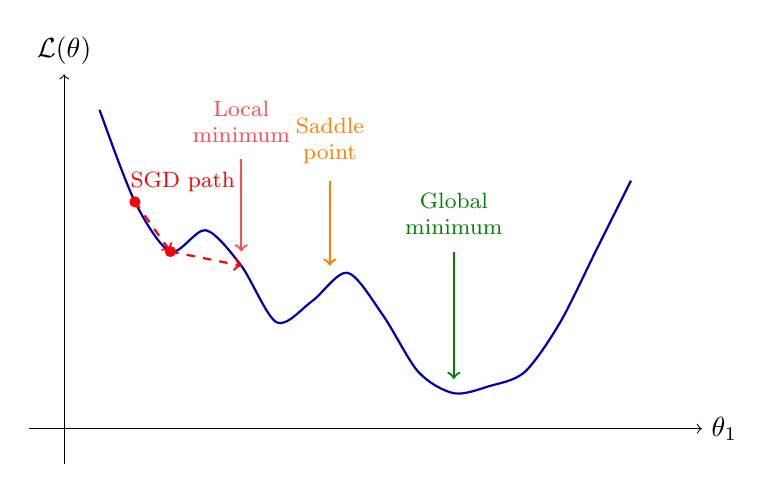
\begin{tikzpicture}[scale=0.9]
  % Draw a stylized loss landscape
  \draw[->] (-0.5, 0) -- (9, 0) node[right] {$\theta_1$};
  \draw[->] (0, -0.5) -- (0, 5) node[above] {$\mathcal{L}(\theta)$};

  % Loss surface with local and global minima
  \draw[thick, blue!70!black, smooth] plot coordinates {
    (0.5, 4.5) (1, 3.2) (1.5, 2.5) (2, 2.8) (2.5, 2.3)
    (3, 1.5) (3.5, 1.8) (4, 2.2) (4.5, 1.6) (5, 0.8)
    (5.5, 0.5) (6, 0.6) (6.5, 0.8) (7, 1.5) (7.5, 2.5) (8, 3.5)
  };

  % Label minima
  \draw[->, thick, red!70] (2.5, 3.8) -- (2.5, 2.5);
  \node[above, red!70, font=\footnotesize, align=center] at (2.5, 3.9) {Local\\minimum};

  \draw[->, thick, green!50!black] (5.5, 2.5) -- (5.5, 0.7);
  \node[above, green!50!black, font=\footnotesize, align=center] at (5.5, 2.6) {Global\\minimum};

  % Saddle point
  \draw[->, thick, orange] (3.75, 3.5) -- (3.75, 2.3);
  \node[above, orange, font=\footnotesize, align=center] at (3.75, 3.6) {Saddle\\point};

  % SGD trajectory
  \filldraw[red] (1, 3.2) circle (2pt);
  \draw[->, red, thick, dashed] (1, 3.2) -- (1.5, 2.5);
  \filldraw[red] (1.5, 2.5) circle (2pt);
  \draw[->, red, thick, dashed] (1.5, 2.5) -- (2.5, 2.3);
  \node[above right, red, font=\footnotesize] at (0.8, 3.2) {SGD path};
\end{tikzpicture}
\end{center}

Key features of neural network loss landscapes:
\begin{itemize}[leftmargin=1.5em]
  \item \textbf{Local minima} are points where the loss is lower than all nearby points but not the global minimum. In high-dimensional spaces, most local minima have loss values close to the global minimum \citep{goodfellow2016}.
  \item \textbf{Saddle points} are far more common than local minima in high dimensions. At a saddle point, the gradient is zero, but the Hessian has both positive and negative eigenvalues (loss increases in some directions and decreases in others).
  \item \textbf{Plateaus} are flat regions where the gradient is near zero, causing slow learning. Momentum helps escape plateaus by accumulating velocity from previous gradients.
\end{itemize}

\subsection{Regularization: Preventing Overfitting}

A model that memorizes the training data (overfitting) fails to generalize. Regularization techniques constrain the model to prefer simpler solutions:

\begin{enumerate}[leftmargin=1.5em]
  \item \textbf{L2 regularization (weight decay):} Add $\lambda \|\theta\|^2$ to the loss, penalizing large weights:
  \begin{equation}
  \mathcal{L}_{\text{reg}} = \mathcal{L}_{\text{data}} + \lambda \sum_i \theta_i^2.
  \end{equation}
  This is equivalent to a Gaussian prior on the weights in a Bayesian framework. Concretely, $\lambda = 0.01$ means we are saying ``we believe the weights should be small, with a prior variance of $1/(2\lambda) = 50$.'' Larger $\lambda$ imposes a stronger prior, yielding a simpler model.

  \item \textbf{Dropout} \citep{srivastava2014}: During training, randomly set each neuron's output to zero with probability $p$ (typically $p = 0.1$ to $0.5$). This forces the network to learn redundant representations, preventing co-adaptation of neurons. At test time, all neurons are active but outputs are scaled by $(1-p)$ to compensate. Dropout can be interpreted as training an ensemble of $2^N$ sub-networks (where $N$ is the number of neurons) that share parameters.

  \item \textbf{Early stopping:} Monitor performance on a held-out validation set and stop training when validation loss begins to increase, even if training loss continues to decrease. The gap between training loss (decreasing) and validation loss (increasing) is a signature of overfitting.

  \item \textbf{Data augmentation:} Artificially increase the training set by applying transformations. For DNA sequences, augmentations include reverse complementation, random mutation, and subsequence extraction.

  \item \textbf{Layer normalization} \citep{ba2016}: Normalize activations within each layer to have zero mean and unit variance, stabilizing the distribution of hidden representations. For a vector $\mathbf{h}$ of activations: $\text{LayerNorm}(\mathbf{h}) = \gamma \cdot \frac{\mathbf{h} - \mu}{\sqrt{\sigma^2 + \epsilon}} + \beta$, where $\mu$ and $\sigma^2$ are the mean and variance of $\mathbf{h}$, and $\gamma, \beta$ are learned scale and shift parameters.
\end{enumerate}

\begin{bioinsight}[Gradient Descent vs.\ Evolution]
Gradient descent optimizes parameters along the loss landscape using local gradient information. Evolution optimizes genomes through population-based search using fitness evaluation. The table below highlights key differences:
\begin{center}
\renewcommand{\arraystretch}{1.12}
\begin{tabularx}{0.85\textwidth}{L{3cm} L{3.5cm} Y}
\toprule
\textbf{Property} & \textbf{Gradient Descent} & \textbf{Evolution} \\
\midrule
Search signal & Gradient (local) & Fitness (global) \\
Update rule & Continuous, small steps & Discrete mutations \\
Parallelism & Mini-batch & Population \\
Exploration & Limited (local minima) & Broad (mutation diversity) \\
Requires & Differentiable loss & Only evaluable fitness \\
State & Parameters ($\mathbb{R}^d$) & Genomes (structured) \\
Memory & None (memoryless) & Population history \\
\bottomrule
\end{tabularx}
\end{center}
DOGMA uses both: gradient descent for training neural components, and evolutionary search for optimizing prompt genomes and architectural structure (Chapter~\ref{ch:evolutionary-training}).
\end{bioinsight}

% ───────────────────────────────────────────────────────────────────────────────
\section{Convolutional Neural Networks}
\label{sec:cnns}

Before transformers dominated, \emph{convolutional neural networks} (CNNs) were the architecture of choice for structured data. CNNs remain important in biological AI for processing DNA sequences and protein structures.

\subsection{The Convolution Operation}

A 1D convolution slides a learned filter (kernel) $\mathbf{k} \in \mathbb{R}^w$ across an input sequence $\mathbf{x} \in \mathbb{R}^T$ to produce a feature map:
\begin{equation}
(\mathbf{x} * \mathbf{k})_t = \sum_{i=0}^{w-1} k_i \cdot x_{t+i}.
\end{equation}

The convolution has two important properties that make it efficient and effective:
\begin{itemize}[leftmargin=1.5em]
  \item \textbf{Parameter sharing:} The same filter weights are used at every position. A filter with width $w$ has only $w$ parameters regardless of sequence length $T$, compared to $T \times T$ for a fully connected layer.
  \item \textbf{Translation equivariance:} If the input shifts by $k$ positions, the output feature map also shifts by $k$ positions. A motif detector works identically regardless of where the motif appears in the sequence.
\end{itemize}

\paragraph{Worked example: motif detection in DNA.} Suppose we have a DNA sequence encoded numerically: $\mathbf{x} = [1, 0, 0, 1, 1, 0, 1, 0]$ (where 1 = purine, 0 = pyrimidine). A filter $\mathbf{k} = [1, 1, 1]$ (width 3) detects runs of three purines:
\begin{align}
(\mathbf{x} * \mathbf{k})_1 &= 1 \cdot 1 + 0 \cdot 1 + 0 \cdot 1 = 1 \\
(\mathbf{x} * \mathbf{k})_2 &= 0 \cdot 1 + 0 \cdot 1 + 1 \cdot 1 = 1 \\
(\mathbf{x} * \mathbf{k})_3 &= 0 \cdot 1 + 1 \cdot 1 + 1 \cdot 1 = 2 \\
(\mathbf{x} * \mathbf{k})_4 &= 1 \cdot 1 + 1 \cdot 1 + 0 \cdot 1 = 2 \\
(\mathbf{x} * \mathbf{k})_5 &= 1 \cdot 1 + 0 \cdot 1 + 1 \cdot 1 = 2 \\
(\mathbf{x} * \mathbf{k})_6 &= 0 \cdot 1 + 1 \cdot 1 + 0 \cdot 1 = 1
\end{align}
The highest activations (value 2) occur at positions 3--5, where purine density is highest. In practice, DNA models like DeepSEA \citep{zhou2015} use hundreds of learned filters to detect regulatory motifs.

\subsection{Key CNN Concepts}

\begin{itemize}[leftmargin=1.5em]
  \item \textbf{Stride:} The step size between filter applications. Stride $>1$ reduces output length (downsampling). With stride $s$, an input of length $T$ with filter width $w$ produces an output of length $\lfloor (T - w)/s \rfloor + 1$.
  \item \textbf{Padding:} Adding zeros around the input to control output size. ``Same'' padding preserves input length; ``valid'' padding (no padding) reduces length by $w - 1$.
  \item \textbf{Pooling:} Aggregating neighboring activations (max pooling or average pooling) to reduce dimensionality and provide translation invariance. Max pooling with window 2 halves the sequence length while keeping the strongest activations.
  \item \textbf{Multiple channels:} Each input can have multiple channels (e.g., 4 channels for one-hot encoded DNA), and each filter produces one output channel. A CNN layer with $C_{\text{in}}$ input channels and $C_{\text{out}}$ filters has $C_{\text{out}} \times C_{\text{in}} \times w$ learnable weights.
  \item \textbf{Dilated convolutions:} Inserting gaps between filter elements allows a small filter to cover a large receptive field. A filter with dilation $d$ and width $w$ has an effective receptive field of $w + (w-1)(d-1)$ positions. This is useful for capturing long-range patterns in DNA without increasing parameters.
\end{itemize}

\paragraph{Receptive field growth.} Stacking $L$ convolutional layers with filter width $w$ gives a total receptive field of $L(w-1) + 1$. With dilated convolutions using dilation rates $1, 2, 4, \ldots, 2^{L-1}$, the receptive field grows exponentially as $2^L - 1 + w - 1$. For DNA, where regulatory elements can influence expression from thousands of bases away, this exponential growth is essential.

\begin{keyinsight}[CNNs in DOGMA]
DOGMA's strand displacement computational path (Chapter~\ref{ch:dogma-architecture}) is conceptually related to 1D convolution: it slides local operations along the genomic sequence, detecting and transforming local patterns. However, DOGMA adds \emph{typed} convolution: the operation depends on the base types being processed, analogous to how different enzymes recognize different DNA motifs.
\end{keyinsight}

% ───────────────────────────────────────────────────────────────────────────────
\section{Representation Learning}
\label{sec:representation-learning}

\subsection{Embeddings: Mapping Symbols to Geometry}

The core idea of representation learning is to map discrete symbols into continuous vector spaces where geometric relationships capture semantic relationships. An \emph{embedding} is a learned function $e : \Sigma \to \mathbb{R}^d$ that assigns each symbol a dense vector.

For a vocabulary $V$ of size $|V|$, an embedding layer is a matrix $\mathbf{E} \in \mathbb{R}^{|V| \times d}$ where row $i$ is the embedding of token $i$. The embedding is learned end-to-end through backpropagation.

Why embeddings rather than one-hot encoding? A one-hot vector for a vocabulary of size $|V|$ is $|V|$-dimensional with a single 1 and all other entries 0. This representation has several problems: (1) it is very high-dimensional for large vocabularies ($|V| = 64$ for DNA 3-mers, $|V| \approx 50{,}000$ for text), (2) all pairs of symbols are equidistant (cosine similarity is 0 between any two different one-hot vectors), so the representation encodes no similarity structure, and (3) it is extremely sparse. Embeddings solve all three problems: they are low-dimensional ($d \ll |V|$), they capture similarity (similar symbols have similar embeddings), and they are dense.

\paragraph{Worked example: DNA k-mer embeddings.} Consider a vocabulary of all DNA 3-mers (64 possible): ATG, AAA, CCC, etc. An embedding dimension of $d = 16$ gives an embedding matrix $\mathbf{E} \in \mathbb{R}^{64 \times 16}$. After training on genomic data, we might find:
\begin{itemize}[leftmargin=1.5em]
  \item Start codons (ATG) and other coding-related 3-mers cluster together.
  \item GC-rich 3-mers (GCG, CGC, GGC) cluster separately from AT-rich 3-mers (AAT, TAT, ATA).
  \item Reverse complement pairs (e.g., ATG and CAT) have related but not identical embeddings.
\end{itemize}

The embedding captures both chemical properties (GC content) and functional properties (coding vs.\ regulatory) without being explicitly told about either.

\paragraph{Worked example: cosine similarity computation.} Suppose after training, the embeddings (simplified to $d = 4$) are: ATG $= [0.8, 0.3, -0.1, 0.5]$ and GTG $= [0.7, 0.4, -0.2, 0.6]$. The cosine similarity is:
\begin{align}
\mathbf{u} \cdot \mathbf{v} &= 0.8 \times 0.7 + 0.3 \times 0.4 + (-0.1)(-0.2) + 0.5 \times 0.6 = 0.56 + 0.12 + 0.02 + 0.30 = 1.00 \\
\|\mathbf{u}\| &= \sqrt{0.64 + 0.09 + 0.01 + 0.25} = \sqrt{0.99} \approx 0.995 \\
\|\mathbf{v}\| &= \sqrt{0.49 + 0.16 + 0.04 + 0.36} = \sqrt{1.05} \approx 1.025 \\
\text{sim}(\mathbf{u}, \mathbf{v}) &= \frac{1.00}{0.995 \times 1.025} \approx 0.980.
\end{align}
The high similarity ($0.98$) reflects that ATG and GTG are functionally related---both are alternative start codons in some organisms.

\begin{keyinsight}[Embeddings in DOGMA]
DOGMA's genomic bases carry embeddings as their content component $\sigma_i$, but they also carry \emph{type} ($\tau_i$), \emph{regulatory weight} ($\rho_i$), and \emph{compatibility state} ($\omega_i$). Formally, each base is a tuple $b_i = (\sigma_i, \tau_i, \rho_i, \omega_i)$. This is richer than a standard token embedding because each base is not merely a point in semantic space---it is a typed, weighted, interaction-annotated computational atom.
\end{keyinsight}

\subsection{The Geometry of Meaning}

Good embeddings exhibit meaningful geometric structure. Classic examples include Word2Vec's vector arithmetic: $\text{king} - \text{man} + \text{woman} \approx \text{queen}$.

For biological sequences, protein language models learn embeddings where proteins with similar function cluster together, even without explicit functional labels \citep{lin2023}. DNA language models learn embeddings where regulatory elements cluster by function, coding regions by gene family, and promoters by expression level \citep{ji2021dnabert}.

\paragraph{Measuring embedding quality.} Common metrics include:
\begin{itemize}[leftmargin=1.5em]
  \item \textbf{Cosine similarity:} $\text{sim}(\mathbf{u}, \mathbf{v}) = \frac{\mathbf{u} \cdot \mathbf{v}}{\|\mathbf{u}\| \|\mathbf{v}\|}$. Values near 1 indicate similar vectors.
  \item \textbf{k-nearest neighbors accuracy:} What fraction of an embedding's $k$ nearest neighbors share its class label?
  \item \textbf{Linear probing:} Train a linear classifier on frozen embeddings. High accuracy indicates the embeddings capture relevant structure. For example, if a linear probe on DNABERT embeddings can predict whether a sequence is a promoter with 85\% accuracy, the embeddings have learned promoter-relevant features even though the model was never trained on promoter labels.
\end{itemize}

\subsection{Positional Encoding}

Embeddings alone do not capture \emph{position}---``ATG at position 1'' and ``ATG at position 100'' have identical embeddings. Positional encoding injects position information:

\begin{equation}
\text{PE}(pos, 2i) = \sin\!\left(\frac{pos}{10000^{2i/d}}\right), \quad
\text{PE}(pos, 2i+1) = \cos\!\left(\frac{pos}{10000^{2i/d}}\right).
\end{equation}

These sinusoidal functions create unique position-dependent patterns. The frequency decreases with dimension index $i$, so the first dimensions encode fine-grained position and later dimensions encode coarser position.

\paragraph{Why sinusoidal?} The sinusoidal encoding has two useful properties. First, each position gets a unique encoding (no two positions have the same pattern across all dimensions). Second, the encoding supports relative position computation: for any fixed offset $k$, $\text{PE}(pos + k)$ can be expressed as a linear function of $\text{PE}(pos)$, allowing the model to learn attention patterns that depend on relative position. An alternative is \emph{learned} positional embeddings, which train a separate embedding vector for each position. Learned embeddings are more flexible but cannot extrapolate to positions longer than seen during training.

\begin{bioinsight}[Positional Encoding and Genomic Coordinates]
In biology, position matters enormously: the same sequence TATAAA functions as a promoter only at specific distances upstream of a gene. DOGMA's genomic bases encode position implicitly through their region membership and regulatory context, rather than through additive positional encoding. This is more biologically realistic: a cell does not ``add'' a position signal to each nucleotide; instead, the 3D structure of chromatin determines which regions are accessible.
\end{bioinsight}

% ───────────────────────────────────────────────────────────────────────────────
\section{Sequence Models: From RNNs to State Spaces}
\label{sec:sequence-models}

Biological data is inherently sequential: DNA sequences, protein chains, gene expression time series. Sequence models are therefore central to biological AI.

\subsection{Recurrent Neural Networks}

RNNs process sequences by maintaining a hidden state $\mathbf{h}_t$ that is updated at each time step:
\begin{equation}
\mathbf{h}_t = \phi(\mathbf{W}_h \mathbf{h}_{t-1} + \mathbf{W}_x \mathbf{x}_t + \mathbf{b}).
\end{equation}

The hidden state acts as a ``memory'' that accumulates information from previous time steps. At each step, the RNN takes the current input $\mathbf{x}_t$ and the previous hidden state $\mathbf{h}_{t-1}$, combines them through a linear transformation, applies a nonlinearity, and produces a new hidden state $\mathbf{h}_t$. This hidden state serves two purposes: it is the representation used for prediction at time $t$, and it is the memory passed to time $t+1$.

However, vanilla RNNs struggle with long sequences due to the \emph{vanishing gradient problem}: gradients shrink exponentially as they propagate backward through many time steps.

\paragraph{Vanishing gradients: a concrete example.} If the gradient at each time step is multiplied by a factor $\alpha < 1$, then after $T$ steps the gradient is $\alpha^T$. For $\alpha = 0.9$ and $T = 100$: $0.9^{100} \approx 2.7 \times 10^{-5}$. The gradient has effectively vanished, making it impossible to learn long-range dependencies. For DNA sequences, which can be hundreds of thousands of bases long, this is catastrophic: an RNN cannot learn that a promoter 10,000 bases upstream affects a gene's expression.

\subsection{Long Short-Term Memory (LSTM)}

The LSTM architecture \citep{hochreiter1997} addresses vanishing gradients by adding a \emph{cell state} $\mathbf{c}_t$ that flows through time with minimal transformation, gated by three learned gates:

\begin{align}
\mathbf{f}_t &= \sigma(\mathbf{W}_f [\mathbf{h}_{t-1}, \mathbf{x}_t] + \mathbf{b}_f) & \text{(forget gate)} \\
\mathbf{i}_t &= \sigma(\mathbf{W}_i [\mathbf{h}_{t-1}, \mathbf{x}_t] + \mathbf{b}_i) & \text{(input gate)} \\
\tilde{\mathbf{c}}_t &= \tanh(\mathbf{W}_c [\mathbf{h}_{t-1}, \mathbf{x}_t] + \mathbf{b}_c) & \text{(candidate cell state)} \\
\mathbf{c}_t &= \mathbf{f}_t \odot \mathbf{c}_{t-1} + \mathbf{i}_t \odot \tilde{\mathbf{c}}_t & \text{(cell state update)} \\
\mathbf{o}_t &= \sigma(\mathbf{W}_o [\mathbf{h}_{t-1}, \mathbf{x}_t] + \mathbf{b}_o) & \text{(output gate)} \\
\mathbf{h}_t &= \mathbf{o}_t \odot \tanh(\mathbf{c}_t) & \text{(hidden state)}
\end{align}

where $\odot$ denotes element-wise multiplication and $[\cdot, \cdot]$ denotes concatenation.

The key idea is the cell state $\mathbf{c}_t$: information flows along the cell state with only multiplicative gating (the forget gate $\mathbf{f}_t$) and additive updates (the input gate $\mathbf{i}_t \odot \tilde{\mathbf{c}}_t$). If the forget gate is close to 1 and the input gate close to 0, information is preserved indefinitely. This creates a ``gradient highway'' that allows gradients to flow backward through time without shrinking.

\begin{bioinsight}[LSTM Gates and Biological Regulation]
The LSTM's gating mechanism has a striking parallel to gene regulation:
\begin{center}
\renewcommand{\arraystretch}{1.12}
\begin{tabularx}{0.9\textwidth}{L{3cm} L{3.5cm} Y}
\toprule
\textbf{LSTM Component} & \textbf{Biological Analogue} & \textbf{Function} \\
\midrule
Forget gate $\mathbf{f}_t$ & Silencer element & Suppresses previously stored information \\
Input gate $\mathbf{i}_t$ & Promoter/enhancer & Controls which new information to store \\
Output gate $\mathbf{o}_t$ & Transcription regulation & Controls which information to express \\
Cell state $\mathbf{c}_t$ & Epigenetic memory & Persistent information across time \\
\bottomrule
\end{tabularx}
\end{center}
DOGMA's regulation stage generalizes this parallel into a full architectural principle with typed bases and region-level control. Rather than three gates operating on a single vector, DOGMA applies context-dependent activation weights to entire genomic regions with rich type information.
\end{bioinsight}

\subsection{State Space Models}

An emerging alternative to attention-based sequence models is the \emph{structured state space model} (SSM) \citep{gu2022s4, gu2023mamba}. SSMs process sequences through a linear dynamical system:

\begin{align}
\mathbf{h}_t &= \mathbf{A} \mathbf{h}_{t-1} + \mathbf{B} \mathbf{x}_t, \label{eq:ssm-state} \\
\mathbf{y}_t &= \mathbf{C} \mathbf{h}_t + \mathbf{D} \mathbf{x}_t, \label{eq:ssm-output}
\end{align}

where $\mathbf{A}, \mathbf{B}, \mathbf{C}, \mathbf{D}$ are structured matrices. The key innovation of SSMs is that the recurrence in Equation~\ref{eq:ssm-state} can be computed as a \emph{convolution} during training (enabling parallelism) and as a \emph{recurrence} during inference (enabling efficient autoregressive generation).

\paragraph{Why the dual computation matters.} To see how the recurrence becomes a convolution, unroll the state equation:
\begin{align}
\mathbf{h}_0 &= \mathbf{B}\mathbf{x}_0, \\
\mathbf{h}_1 &= \mathbf{A}\mathbf{B}\mathbf{x}_0 + \mathbf{B}\mathbf{x}_1, \\
\mathbf{h}_2 &= \mathbf{A}^2\mathbf{B}\mathbf{x}_0 + \mathbf{A}\mathbf{B}\mathbf{x}_1 + \mathbf{B}\mathbf{x}_2.
\end{align}
The output $\mathbf{y}_t = \mathbf{C}\mathbf{h}_t$ depends on all past inputs through the kernel $\bar{K}_t = \mathbf{C}\mathbf{A}^t\mathbf{B}$, yielding $\mathbf{y} = \bar{K} * \mathbf{x}$---a convolution that can be computed in $O(T \log T)$ via FFT during training. During inference, only one step of the recurrence is needed per token, giving $O(1)$ per-token cost.

\paragraph{Complexity comparison.}
\begin{center}
\renewcommand{\arraystretch}{1.12}
\begin{tabularx}{0.85\textwidth}{L{3.5cm} L{3cm} Y}
\toprule
\textbf{Architecture} & \textbf{Training} & \textbf{Inference (per token)} \\
\midrule
RNN / LSTM & $O(T)$ sequential & $O(1)$ \\
Transformer & $O(T^2)$ parallel & $O(T)$ (KV cache) \\
SSM (S4/Mamba) & $O(T \log T)$ parallel & $O(1)$ \\
\bottomrule
\end{tabularx}
\end{center}

The Mamba architecture \citep{gu2023mamba} makes the SSM matrices \emph{input-dependent}, achieving selective state-space modeling: the model can choose which information to remember or forget based on the input, similar to LSTM gating but with $O(T)$ complexity.

\begin{keyinsight}[SSMs in DOGMA]
DOGMA's ParallelScan computational path implements a variant of selective state-space processing. The state transition matrix $\mathbf{A}$ is parameterized using thermodynamic binding energies from the SantaLucia nearest-neighbor model, providing a biophysically grounded state dynamics. This provides linear-time sequence processing for long genomic sequences while maintaining biological interpretability.
\end{keyinsight}

% ───────────────────────────────────────────────────────────────────────────────
\section{Evolutionary Algorithms}
\label{sec:evolutionary-algorithms}

Evolutionary algorithms (EAs) are optimization methods inspired by biological evolution \citep{holland1975, dejong2006}. They maintain a \emph{population} of candidate solutions and iteratively apply \emph{selection}, \emph{mutation}, and \emph{recombination} to improve population fitness.

\subsection{The Genetic Algorithm: Step by Step}

A standard genetic algorithm (GA) proceeds through the following steps:

\begin{enumerate}[leftmargin=1.5em]
  \item \textbf{Initialize:} Create a random population of $N$ candidate solutions (``individuals''), each encoded as a genome (e.g., a bit string, a real-valued vector, or a structured object).

  \item \textbf{Evaluate:} Compute a fitness score $f(\mathbf{x}_i)$ for each individual $\mathbf{x}_i$.

  \item \textbf{Select parents:} Choose individuals for reproduction, with probability proportional to fitness. Common selection methods:
  \begin{itemize}[leftmargin=1.5em]
    \item \emph{Tournament selection:} Randomly pick $k$ individuals; the fittest wins.
    \item \emph{Roulette wheel:} Select with probability $p_i = f(\mathbf{x}_i) / \sum_j f(\mathbf{x}_j)$.
    \item \emph{Rank selection:} Sort by fitness; select by rank rather than raw fitness value.
  \end{itemize}

  \item \textbf{Crossover (recombination):} Combine two parents to produce offspring:
  \begin{itemize}[leftmargin=1.5em]
    \item \emph{One-point crossover:} Choose a random split point; child gets first part from parent A and second part from parent B.
    \item \emph{Uniform crossover:} For each gene, randomly choose from parent A or B.
  \end{itemize}

  \item \textbf{Mutate:} Randomly modify offspring with small probability $p_m$ (e.g., flip a bit, add Gaussian noise to a real-valued gene).

  \item \textbf{Replace:} Form the next generation. Options include generational replacement (all individuals replaced) or steady-state (only a few replaced per iteration).

  \item \textbf{Repeat} steps 2--6 until convergence or a computational budget is exhausted.
\end{enumerate}

% TikZ diagram: Evolutionary algorithm cycle
\begin{center}
\begin{tikzpicture}[
    box/.style={rectangle, draw, rounded corners, minimum width=2.5cm, minimum height=1cm, thick, fill=green!8, align=center},
    arrow/.style={->, thick, >=stealth},
    scale=0.9
]
  % Nodes arranged in a cycle
  \node[box] (init) at (0, 3) {Initialize\\Population};
  \node[box] (eval) at (4, 3) {Evaluate\\Fitness};
  \node[box] (select) at (7, 0.5) {Select\\Parents};
  \node[box] (cross) at (4, -2) {Crossover};
  \node[box] (mutate) at (0, -2) {Mutate};
  \node[box] (replace) at (-3, 0.5) {Replace\\Generation};

  % Check node
  \node[diamond, draw, thick, fill=yellow!15, minimum width=1.5cm, align=center, inner sep=1pt, font=\small] (check) at (-3, 3) {Done?};

  % Arrows
  \draw[arrow] (init) -- (eval);
  \draw[arrow] (eval) -- (select);
  \draw[arrow] (select) -- (cross);
  \draw[arrow] (cross) -- (mutate);
  \draw[arrow] (mutate) -- (replace);
  \draw[arrow] (replace) -- (check);
  \draw[arrow] (check) -- node[above, font=\small] {No} (init);
  \draw[arrow] (check) -- +(-2, 0) node[left, font=\small] {Yes: return best};
\end{tikzpicture}
\end{center}

\paragraph{Worked example: evolving a 6-bit binary string.} Suppose our fitness function counts the number of 1-bits (the ``OneMax'' problem). We want to find the string $111111$.

\begin{enumerate}[leftmargin=1.5em]
\item \textbf{Generation 0 (initialize):} Random population of $N=4$:
\begin{center}
\begin{tabular}{lcc}
\toprule
\textbf{Individual} & \textbf{Genome} & \textbf{Fitness} \\
\midrule
$\mathbf{x}_1$ & 100110 & 3 \\
$\mathbf{x}_2$ & 011001 & 3 \\
$\mathbf{x}_3$ & 110100 & 3 \\
$\mathbf{x}_4$ & 001011 & 3 \\
\bottomrule
\end{tabular}
\end{center}

\item \textbf{Selection (tournament, $k=2$):}
  \begin{itemize}
    \item Pair 1: $\mathbf{x}_1$ (3) vs $\mathbf{x}_3$ (3) $\to$ $\mathbf{x}_3$ wins (tie-break).
    \item Pair 2: $\mathbf{x}_2$ (3) vs $\mathbf{x}_4$ (3) $\to$ $\mathbf{x}_2$ wins.
  \end{itemize}

\item \textbf{Crossover (one-point at position 3):}
  \begin{itemize}
    \item Parent $\mathbf{x}_3 = \mathbf{110}|100$, Parent $\mathbf{x}_2 = \mathbf{011}|001$
    \item Child 1: $110|001 = 110001$ (fitness 3)
    \item Child 2: $011|100 = 011100$ (fitness 3)
  \end{itemize}

\item \textbf{Mutation ($p_m = 0.1$ per bit):} Suppose bit 6 of child 1 flips: $110001 \to 110011$ (fitness 4). Child 2 has no mutations.

\item \textbf{Generation 1:} Replace worst two individuals. New population: $\{110100, 011001, 110011, 011100\}$. Best fitness improved from 3 to 4.
\end{enumerate}

After several more generations, mutation and crossover create individuals with progressively more 1-bits until the optimum $111111$ is found. Note that no gradient was computed---the search is guided entirely by fitness evaluation and random variation.

\paragraph{Worked example: evolving a DNA promoter score.} Suppose we want to find a 10-base DNA sequence that maximizes a promoter strength predictor $f : \{A,C,G,T\}^{10} \to [0,1]$. We initialize a population of $N = 50$ random sequences, evaluate each with the predictor, apply tournament selection ($k=3$), one-point crossover, and point mutations (each base mutated with probability $p_m = 0.05$). After 100 generations, the population converges toward high-scoring promoter sequences---without ever computing a gradient.

\subsection{Quality-Diversity Algorithms}

Standard optimization seeks a single best solution. \emph{Quality-diversity} (QD) algorithms seek a diverse collection of high-quality solutions that cover the space of possible behaviors \citep{mouret2015}.

\begin{dogmadef}[MAP-Elites]
MAP-Elites maintains a grid of behavioral niches, indexed by a \emph{behavioral descriptor} (BD). For each niche, only the best-performing individual is stored. The algorithm:
\begin{enumerate}[leftmargin=1.5em]
  \item Randomly generate initial individuals and place in grid by BD.
  \item Select a random occupied niche; mutate its occupant.
  \item Evaluate the mutant's fitness and BD.
  \item If the mutant's niche is empty or the mutant beats the current occupant, insert it.
  \item Repeat until the grid is filled with diverse, high-quality solutions.
\end{enumerate}
\end{dogmadef}

\paragraph{Intuition for MAP-Elites.} Consider designing DNA aptamers (short DNA sequences that bind to specific targets). The behavioral descriptor might be a 2D space: (GC content, predicted secondary structure stability). MAP-Elites would fill a grid where each cell contains the best-binding aptamer with that particular GC content and stability combination. This gives the designer a menu of high-quality options spanning different properties---far more useful than a single ``best'' aptamer.

\emph{Novelty search} \citep{lehman2011} abandons explicit fitness objectives entirely, rewarding solutions that are behaviorally different from previously encountered ones. This can discover solutions that objective-driven search misses due to deceptive fitness landscapes.

\begin{keyinsight}[Evolutionary Algorithms in DOGMA]
DOGMA's evolutionary training loop (Chapter~\ref{ch:evolutionary-training}) combines multiple EA principles:
\begin{itemize}[leftmargin=1.5em]
  \item \textbf{Mutation:} Prompt genome fragments are modified through targeted edits (point mutations, insertions, deletions, region swaps).
  \item \textbf{Selection:} Multi-objective fitness evaluation using Pareto dominance selects improvements.
  \item \textbf{Novelty:} HelixHash novelty scoring (Chapter~\ref{ch:helixhash}) prevents premature convergence by measuring structural novelty.
  \item \textbf{Quality-diversity:} The HelixHash archive maintains diverse structural variants, analogous to MAP-Elites.
  \item \textbf{Meta-learning:} Cross-run meta-policy memory enables the system to improve at evolving itself---learning which mutation strategies work best in which contexts.
\end{itemize}
\end{keyinsight}

% ───────────────────────────────────────────────────────────────────────────────
\section{Multi-Objective Optimization}
\label{sec:ml-multi-objective}

Real-world learning problems rarely have a single objective. DOGMA's training loop simultaneously optimizes accuracy, schema compliance, distillation agreement, efficiency, and latency.

\subsection{Pareto Optimality}

\begin{definition}[Pareto Dominance and Optimality]
Given two solutions $\mathbf{x}$ and $\mathbf{y}$ evaluated on $m$ objectives $f_1, \ldots, f_m$ (all to be maximized):
\begin{itemize}[leftmargin=1.5em]
  \item $\mathbf{x}$ \emph{Pareto dominates} $\mathbf{y}$ (written $\mathbf{x} \succ \mathbf{y}$) if $f_i(\mathbf{x}) \geq f_i(\mathbf{y})$ for all $i$ and $f_j(\mathbf{x}) > f_j(\mathbf{y})$ for at least one $j$.
  \item $\mathbf{x}$ is \emph{Pareto optimal} if no feasible solution dominates it.
  \item The set of all Pareto-optimal solutions is the \emph{Pareto front}.
\end{itemize}
\end{definition}

\paragraph{Worked example.} Consider three genomes evaluated on accuracy ($f_1$) and efficiency ($f_2$):
\begin{center}
\begin{tabular}{lcc}
\toprule
\textbf{Genome} & \textbf{Accuracy} ($f_1$) & \textbf{Efficiency} ($f_2$) \\
\midrule
$\mathcal{B}_A$ & 0.95 & 0.60 \\
$\mathcal{B}_B$ & 0.85 & 0.90 \\
$\mathcal{B}_C$ & 0.80 & 0.55 \\
\bottomrule
\end{tabular}
\end{center}

$\mathcal{B}_A$ and $\mathcal{B}_B$ are both Pareto optimal---neither dominates the other ($A$ is better on accuracy, $B$ on efficiency). $\mathcal{B}_C$ is dominated by $\mathcal{B}_B$ (worse on both objectives), so $C$ is \emph{not} Pareto optimal. Note that $\mathcal{B}_A$ does not dominate $\mathcal{B}_C$ either: although $A$ is better on accuracy ($0.95 > 0.80$) and efficiency ($0.60 > 0.55$), it does dominate $C$ since it is better on \emph{both} objectives. The Pareto front is therefore $\{\mathcal{B}_A, \mathcal{B}_B\}$.

% TikZ diagram: Pareto front
\begin{center}
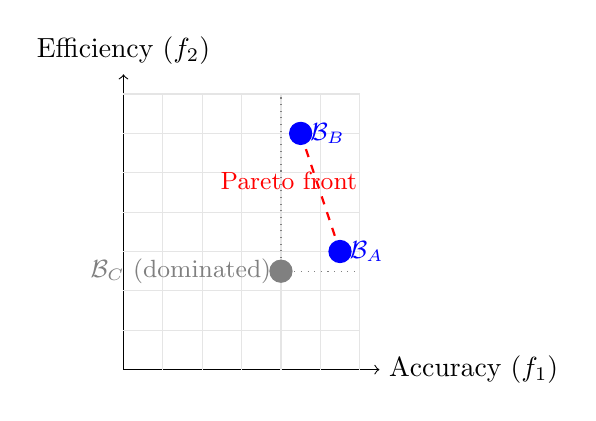
\begin{tikzpicture}[scale=5]
  % Axes
  \draw[->] (0.4, 0.3) -- (1.05, 0.3) node[right] {Accuracy ($f_1$)};
  \draw[->] (0.4, 0.3) -- (0.4, 1.05) node[above] {Efficiency ($f_2$)};

  % Grid lines
  \draw[gray!20] (0.5, 0.3) -- (0.5, 1.0);
  \draw[gray!20] (0.6, 0.3) -- (0.6, 1.0);
  \draw[gray!20] (0.7, 0.3) -- (0.7, 1.0);
  \draw[gray!20] (0.8, 0.3) -- (0.8, 1.0);
  \draw[gray!20] (0.9, 0.3) -- (0.9, 1.0);
  \draw[gray!20] (1.0, 0.3) -- (1.0, 1.0);
  \draw[gray!20] (0.4, 0.4) -- (1.0, 0.4);
  \draw[gray!20] (0.4, 0.5) -- (1.0, 0.5);
  \draw[gray!20] (0.4, 0.6) -- (1.0, 0.6);
  \draw[gray!20] (0.4, 0.7) -- (1.0, 0.7);
  \draw[gray!20] (0.4, 0.8) -- (1.0, 0.8);
  \draw[gray!20] (0.4, 0.9) -- (1.0, 0.9);
  \draw[gray!20] (0.4, 1.0) -- (1.0, 1.0);

  % Pareto front line
  \draw[red, thick, dashed] (0.95, 0.6) -- (0.85, 0.9);

  % Points
  \filldraw[blue] (0.95, 0.6) circle (0.8pt) node[right, font=\small] {$\mathcal{B}_A$};
  \filldraw[blue] (0.85, 0.9) circle (0.8pt) node[right, font=\small] {$\mathcal{B}_B$};
  \filldraw[gray] (0.80, 0.55) circle (0.8pt) node[left, font=\small] {$\mathcal{B}_C$ (dominated)};

  % Dominated region for C
  \draw[gray, dotted] (0.80, 0.55) -- (0.80, 1.0);
  \draw[gray, dotted] (0.80, 0.55) -- (1.0, 0.55);

  % Label
  \node[red, font=\small] at (0.82, 0.78) {Pareto front};
\end{tikzpicture}
\end{center}

\subsection{Scalarization Methods}

The simplest approach to multi-objective optimization is \emph{scalarization}: combine multiple objectives into a single scalar using weights:
\begin{equation}
F_{\text{scalar}}(\mathbf{x}) = \sum_{i=1}^m w_i \cdot f_i(\mathbf{x}), \quad \sum_i w_i = 1.
\end{equation}

The choice of weights $w_i$ determines which point on the Pareto front is found. Different weight vectors trace out different points on the front: $w = [1.0, 0.0]$ finds the solution with maximum accuracy (ignoring efficiency), $w = [0.0, 1.0]$ maximizes efficiency, and $w = [0.5, 0.5]$ seeks a balanced compromise.

DOGMA's multi-objective scoring uses a weighted combination where the weights are \emph{dynamically adjusted} by the Tera regime state (Chapter~\ref{ch:tera}), creating an adaptive scalarization that shifts emphasis based on the current evolutionary pressure landscape.

\begin{equation}
w_i(t) = \text{softmax}\bigl(\mathbf{W}_{\text{tera}} \cdot \mathbf{r}(t) + \mathbf{b}\bigr)_i
\label{eq:ml-tera-weights}
\end{equation}

where $\mathbf{r}(t)$ is the Tera regime state vector at time $t$. When the system is stagnating on accuracy, Tera increases the accuracy weight; when efficiency is lagging, it shifts emphasis to efficiency. This dynamic reweighting is analogous to how biological organisms shift resource allocation under different environmental pressures.

\begin{implnote}
In practice, DOGMA's Tera state smoothly interpolates between weight configurations rather than jumping between them. The softmax temperature is annealed during training: high temperature early on (exploring the full Pareto front) and low temperature later (focusing on the most promising region). This prevents the optimizer from oscillating between objectives and ensures stable convergence.
\end{implnote}

% ───────────────────────────────────────────────────────────────────────────────
\section{Bringing It Together: The DOGMA Learning Stack}
\label{sec:dogma-learning-stack}

The ML concepts introduced in this chapter form the foundation of DOGMA's learning stack. The following table maps each ML concept to its role in DOGMA:

\begin{center}
\renewcommand{\arraystretch}{1.15}
\begin{tabularx}{0.95\textwidth}{L{3.8cm} L{4cm} Y}
\toprule
\textbf{ML Concept} & \textbf{DOGMA Component} & \textbf{Role} \\
\midrule
Embeddings & Genomic base content $\sigma_i$ & Represent symbols as typed vectors \\
Activation functions & Regulatory weights $\rho_i$ & Context-dependent activation \\
CNNs & Strand displacement path & Local pattern detection \\
RNNs/LSTMs & Epigenetic memory (v2) & Persistent state across time \\
SSMs & ParallelScan path & Linear-time sequence processing \\
Backpropagation & Foundation model training & Train neural components \\
Evolutionary search & Evolutionary training loop & Optimize prompt genomes \\
Multi-objective optimization & Tera regime dynamics & Balance competing objectives \\
Quality-diversity & HelixHash archive & Maintain structural diversity \\
Regularization & Type compatibility constraints & Prevent degenerate solutions \\
\bottomrule
\end{tabularx}
\end{center}

This mapping illustrates DOGMA's synthetic approach: rather than choosing between gradient-based and evolutionary optimization, between local and global computation, or between structured and unstructured representations, DOGMA combines the best of each paradigm within a biologically grounded framework.

\begin{keyinsight}[Two-Level Optimization]
DOGMA operates a two-level optimization process that mirrors biology's own dual optimization:
\begin{itemize}[leftmargin=1.5em]
  \item \textbf{Inner loop (gradient descent):} Trains neural network parameters (weights, embeddings) through backpropagation on differentiable losses. This is analogous to \emph{learning within an organism's lifetime}---adjusting synaptic weights through experience.
  \item \textbf{Outer loop (evolutionary search):} Evolves prompt genomes, architectural configurations, and regulatory structures through population-based search. This is analogous to \emph{evolution across generations}---selecting genomes that produce fit organisms.
\end{itemize}
The inner loop handles what is differentiable; the outer loop handles what is not. Together, they cover the full optimization landscape that DOGMA must navigate.
\end{keyinsight}

% ───────────────────────────────────────────────────────────────────────────────
\section{Exercises}
\label{sec:ch4-exercises}

\begin{enumerate}[label=\textbf{4.\arabic*.}, leftmargin=2.5em]

\item \textbf{[Fundamentals]} Derive the gradient of the cross-entropy loss $\mathcal{L} = -\sum_i y_i \log \hat{y}_i$ with respect to the logits $\mathbf{z}$, where $\hat{y}_i = \text{softmax}(\mathbf{z})_i$. Show that the result simplifies to $\hat{\mathbf{y}} - \mathbf{y}$. \emph{Hint:} Start by computing $\partial \hat{y}_i / \partial z_j$ for the cases $i = j$ and $i \neq j$ separately, using the quotient rule on the softmax definition.

\item \textbf{[Coding]} Implement a single-layer neural network from scratch (NumPy only) that classifies DNA 3-mers into categories based on GC content (low: 0--1 G/C, medium: 2, high: 3 G/C). Train with SGD and plot the learning curve. Report final accuracy.

\item \textbf{[Analysis]} Compare the LSTM cell state $\mathbf{c}_t$ with a biological gene's expression level $x_i(t)$ governed by Equation~\ref{eq:grn-dynamics} from Chapter~\ref{ch:gene-regulation}. Identify the biological analogues of the forget gate, input gate, and output gate. Are there regulatory mechanisms that have no LSTM analogue?

\item \textbf{[Backpropagation]} Perform the complete forward and backward pass for a 2-layer MLP with weights $W^{(1)} = \begin{bmatrix} 0.3 & -0.2 \\ 0.4 & 0.1 \end{bmatrix}$, $\mathbf{b}^{(1)} = [0, 0]$, $\mathbf{w}^{(2)} = [0.5, -0.3]$, $b^{(2)} = 0$, input $\mathbf{x} = [1, 2]$, and true label $y = 1$. Use ReLU for the hidden layer and sigmoid for the output. Compute all gradients and the updated weights after one step of SGD with $\eta = 0.1$.

\item \textbf{[Convolutions]} Design a set of 1D convolutional filters (specify the weights) that detect the following DNA motifs: (a) the start codon ATG, (b) any purine-pyrimidine alternating pattern, (c) a CpG dinucleotide. Assume 4-channel one-hot encoded input (A, C, G, T).

\item \textbf{[Theory]} Prove that the Pareto front of a bi-objective optimization problem with convex feasible set is a connected curve. Give a counterexample for non-convex problems.

\item \textbf{[Design]} Design a quality-diversity algorithm for evolving DNA primer sequences. Define the behavioral descriptor space, the quality metric, and the mutation operators. Explain how your design prevents the population from converging prematurely.

\item \textbf{[Research]} Read \citet{hansen2001} on CMA-ES. How does CMA-ES's covariance adaptation relate to DOGMA's Tera regime state adaptation? Both systems learn about the local landscape to guide search---compare their mechanisms.

\item \textbf{[Activation Functions]} Implement sigmoid, ReLU, GELU, and Swish in Python. For each, plot the function and its derivative on $[-5, 5]$. Which derivative has the largest maximum value? Which never saturates?

\item \textbf{[Embeddings]} Train Word2Vec-style embeddings on DNA 4-mers using the skip-gram objective on a small genome (e.g., E.\ coli). Visualize the embeddings using t-SNE. Do reverse complement pairs cluster together?

\item \textbf{[Gradient Descent]} Implement gradient descent on $f(\theta_1, \theta_2) = (\theta_1 - 2)^2 + 10(\theta_2 - \theta_1^2)^2$ (a scaled Rosenbrock function). Starting from $\theta_0 = (-1, 1)$, compare the trajectories of plain SGD ($\eta = 0.001$), SGD with momentum ($\beta = 0.9$), and Adam. Plot the trajectories overlaid on a contour plot of $f$. Which optimizer converges fastest? Why?

\item \textbf{[Evolutionary Algorithms]} Implement a genetic algorithm to find the DNA 8-mer with maximum GC content (trivial optimal: \texttt{GCGCGCGC}). Use tournament selection ($k=2$), uniform crossover, and point mutation ($p_m = 0.1$ per base). Track the population's average and best fitness over 50 generations. How does increasing the population size from $N=10$ to $N=100$ affect convergence speed?

\end{enumerate}

% ───────────────────────────────────────────────────────────────────────────────
\section{Key Takeaways}

\keytakeaway{
\begin{itemize}[leftmargin=1.5em]
  \item Machine learning is function approximation from data; the loss function defines what ``good'' means, and the optimizer finds parameters that minimize loss.
  \item Neural networks gain expressiveness from depth and nonlinearity; the universal approximation theorem guarantees expressiveness, but depth provides efficiency.
  \item Backpropagation computes gradients efficiently via the chain rule; Adam is the standard optimizer for modern deep learning.
  \item Regularization (L2, dropout, early stopping) prevents overfitting by constraining model complexity.
  \item Convolutional networks detect local patterns through learned filters---DOGMA's strand displacement path generalizes this with typed convolution.
  \item Self-supervised learning (next-token prediction) is the dominant paradigm for both language and genomic foundation models.
  \item Representation learning maps discrete symbols to continuous geometry---DOGMA extends this with typed, weighted genomic bases carrying regulatory state.
  \item LSTM gating parallels biological gene regulation; DOGMA generalizes this to full region-level regulatory control.
  \item State space models offer $O(T)$ sequence processing---DOGMA's ParallelScan path adopts this efficiency with biophysical parameterization.
  \item Evolutionary algorithms provide gradient-free optimization---DOGMA combines gradient training with evolutionary prompt genome optimization.
  \item Multi-objective optimization with dynamic Tera-driven weight adaptation enables balanced improvement across competing objectives.
\end{itemize}
}

\section*{Suggested Reading}
\begin{itemize}[leftmargin=1.5em]
  \item \citet{goodfellow2016}: Comprehensive deep learning reference---the standard textbook.
  \item \citet{hochreiter1997}: LSTM---foundational for sequence modeling and gating mechanisms.
  \item \citet{kingma2015}: Adam optimizer---the workhorse of modern deep learning.
  \item \citet{gu2023mamba}: Mamba---selective state spaces as an attention alternative.
  \item \citet{srivastava2014}: Dropout regularization---simple but effective.
  \item \citet{holland1975}: Genetic algorithms---the original EA framework.
  \item \citet{mouret2015}: MAP-Elites---quality-diversity algorithms.
  \item \citet{lehman2011}: Novelty search---objectives are not always necessary.
  \item \citet{ji2021dnabert}: DNABERT---applying BERT to genomic sequences.
  \item \citet{zhou2015}: DeepSEA---CNNs for predicting chromatin effects from DNA sequence.
\end{itemize}
